\%
%
%%%%%%%%%%%%%%%%%%%%%%%%%%%%%%%%%%%%%%%%%%%%%%%%%%%%%%%%%%%%%%%%%%%%%%%%%%%%%%%
% Theory
%%%%%%%%%%%%%%%%%%%%%%%%%%%%%%%%%%%%%%%%%%%%%%%%%%%%%%%%%%%%%%%%%%%%%%%%%%%%%%%
%
%\chapter{Quantum Chromodynamics}
\chapter{The theory of the strong interactions}

%------------------------------------------------------------------------
\section{The Standar Model}\label{sec:qcdintro}
%------------------------------------------------------------------------


%------------------------------------------------------------------------
%\subsection{Quantum Chromodynamics}\label{sec:qcd}
%------------------------------------------------------------------------


%------------------------------------------------------------------------
\section{Jet physics}\label{sec:jets}
%------------------------------------------------------------------------


Due to confinement quarks do not exist in isolation, but rather transform into stable color-singlet hadrons. Consequently, the experimental signature of quarks and gluons are the final state hadrons. The packet of particles produced tends to travel collinearly with the direction of the initiator quark or gluon. The result is a ``spray'' of hadrons (also photons and leptons) entering the detector in place of the original parton; these clusters of objects are what we define as jets.
%using inclusive hadronic event shapes to demonstrate the presence of jets.

The evolution from a single parton to an ensemble of hadrons accurs through the processes of parton showering and hadronization. Since the strong coupling constant grows with increasing distance between color charges, a strong color potential forms as the parton from the ``hard'' (high $Q^2$) scattering process separates from the original hadron. This large potential causes quark$/$antiquark pairs ($q\bar{q}$) to be created, each carrying some of the energy and momentum of the original partons. As these new partons move away from one another, yet more color potentials are formed, and the process repeats. Thus from one parton a shower of partons appears, traveling along the same direction as the original.  This process continues until there is no longer enough energy to create additional $q\bar{q}$ pairs, and instead the remaining partons combine to form stable hadrons. Since this progression involves successively lower energies and lower momentum transfers, perturbative QCD cannot describe the full process.  The hadronization process then cannot be calculated from first principles, but has to be modelled (see next section). 
%In real life (data), fluctuations arise from the quantum mechanics of the underlying theory.  In generators, Monte Carlo (MC) techniques are used to select all relevant variables according to the desired probability distributions, and consecuently ensure (quasi-)randomness in the final state. This is the subject of the next section.
%From Pythia's manual http://arxiv.org/abs/hep-ph/0603175

The first evidence for jet production was observed in $e^+e^-$ collisions at the SPEAR storage ring at SLAC in 1975~\cite{PhysRevLett.35.1609}.

\subsection{Monte Carlo tools}

%In high-energy processes such a those at the LHC, the low value of the strong force coupling constant can be exploited, allowing perturbative techniques to be used to calculate physical processes.  We can use the perturbative language to describe the shoft-distance interactions of quarks, leptons and gauge bosons. For leptons and gauge bosons, that lack of colour charge, this language is adequate. However for the interaction of quark and gluons in hadron collisions, this picture must be completed with the structure of incoming hadrons and a model for the fragmentation and decay (hadronization) process, that cannot be calculated from first principles.

%From Gavins's http://arxiv.org/abs/1011.5131
Knowing QCD predictinos is crucial in the design of methods to search for new physics, as well as for extracting meaning from data. Different techniques can be used to make QCD predictions at hadron colliders, and in particular at the LHC. The so called Matrix Element Monte Carlos use direct perturbative calculations of the cross-section matrix elements in powers of the strong coupling constant, $\alpha_s$, for each relevant partonic subprocesses. Leading order (LO) and next-to-leading order (NLO) calculations are available for many processes.   These ``fixed-order predictions'' include the first terms in the QCD perturbative expansion for a given cross-section; as more terms are involved in the expanstion, an improvement in the accuracy of the prediction is expected.  The complexity of the calculations increased significantly with the number of outgoing legs, limiting available results to those with at most three outgoing partons. Matrix element MC programs include {\sc Alpgen}~\cite{ALPGEN}, {\sc Madgraph}~\cite{MADGRAPH} and others.
%Are these characteristics representative of the ‘typical’ situation for collider observables? We only have predictions up to NNLO in a handful of cases (see below) and in those it is. In cases where wejust have NLO predictions, the features of large ‘K-factors’ (NLO/LO enhancements) with a reduced NLO uncertainty band are not uncommon, suggesting that beyond NLO corrections should be small. Exceptions are known to arise in two types of case: those where new enhanced partonic scattering channels open up at NLO (or beyond); and that involve two disparate physical scales.
%Technically, one main consideration has so far limited the range of processes for which NLO results exist: the availability of the loop amplitude. Until recently loop amplitudes were usually calculated semi-manually for each process. The complexity of the calculations increased significantly with the number of outgoing legs, limiting available results to those with at most three outgoing partons. Many NLO results for 2 → 2 and 2 → 3 processes are incorporated into programs such as NLOJ ET++ for jet production [65], MCFM for processes with heavy quarks and/or heavy electroweak bosons [66]


An alternative approach is applied by the so called Monte Carlo parton shower programs. These simulation programs use LO perturbative calculations of matrix elements for $2 \rightarrow 2$ processes, relying on the parton shower to produce the equivalent of multi-parton final state.  {\sc Pythia}~\cite{PYTHIA6} and {\sc Herwig}$++$~\cite{HerwigPP} are the most commonly used parton shower Monte Carlos together with {\sc SHERPA}. % and others.  
%how to get a parton shower event
%A quantity called Sudakov form factor (P (no emission above kt ) ≡ ∆(kt , Q)) allows us to easily calculate the distribution in transverse momentum of the gluon with largest transverse momentum in an event.
%FORMULA
%This distribution is easy to generate by Monte Carlo methods: take a random number r from a distribution that is uniform in the range 0 < r < 1 and find the kt1 that solves ∆(kt1 , Q) = r. Given kt1 we also need to generate the energy for the gluon, but that’s trivial. If we started from a q q system (with some randomly generated orientation), then this gives us a q q g system. As a next step one can work out the Sudakov form factor in the soft/collinear limit for there to be no emission from the q q g system as a whole above some scale kt2 (< kt1 ) and use this to generate a second gluon. The procedure is then repeated over and over again until you find that the next gluon you would generate is below some non-perturbative cutoff scale Q0 , at which point you stop. This gives you one ‘parton shower’ event.
%The above shower descriptions hold for final-state branching. With initial-state hadrons, one also needs to be careful with the treatment of the PDFs, since the collinear splitting that is accounted for in the parton shower is also connected with the way the PDF is built up at the scale of the hard scattering.


The Monte Carlo generators must account for and correctly model the showering of partons. To approximate the energy-evolution of the shower, the DGLP (REFEERNCIAS?) equations that describe the evolution of the PDFs with changing energy scale can be used. The separation of radiation into initial- (before the hard scattering process takes place) and final-state showers is arbitrary, but sometimes convenient.  In both initial- and final-state showers, the structure is given in terms of branchings $a \rightarrow bc$: $q \rightarrow qg$, $q \rightarrow q\gamma$, $g \rightarrow gg$ and $g \rightarrow q\bar{q}$. Parton $b$ carries a fraction $z$ of the energy of the mother energy and parton $c$ carries the remaining $1-z$ (the term ``partons'' is including the radiated photons).  In turn, daughters $b$ and $c$ may also branch, and so on. Each parton is characterized by some evolution scale, which gives an approximate sense of time ordering to the cascade. In the initial-state shower,  the evolution scale values are gradually increasing as the hard scattering is approached, while  these values decrease in the final-state showers. The evolution variable of the cascade in the case of {\sc Pythia} generator, $Q^2$, has traditionally been associated with the $m^2$ of the branching partons\footnote{The final-state partons have $m^2>0$. For initial-state showers the evolution variable is $Q^2=-m^2$, which is required to be strictly increasing along the shower.}. In the recent version of {\sc Pythia} a $p_{\perp}$-ordered shower algorithm, with $Q^2=p_{\perp}^2$ is available, and the shower evolution is cut off at some lower scale  $Q_0$ typically arond 1 GeV for QCD branchings. {\sc Herwig}$++$ provides a shower model which is angular-ordered.

There are two leading models for the description of the non-perturbative process of hadronization, after parton showering. {\sc Pythia} uses the Lund string model of hadronization to form particles~\cite{LUNDMODEL}.  This model involves stretching a colour ``string'' across quarks and gluons and breaking it up into hadrons.% In this model, the color force felt between partons is described as a string connecting them. When the potential is large enough, the string snaps into two, each broken end links a new parton to the one of the original partons.
{\sc Herwig}$++$ utilizes the cluster model of hadronization. In this model each gluon is split into a $q\bar{q}$ pair and then quarks and anti-quarks are grouped into colourless ``clusters'', which then give the hadrons.

Hadronization models involve a number of ‘non-perturbative’ parameters. The parton-shower itself involves the non-perturbative cut-off $Q^2_0$ . These different parameters are usually tuned to data from the LEP experiments.


In addition to the hard interaction that is generated by the Monte Carlo
simulation, it is also necessary to account for the interactions between the incoming proton  remnants. This is usually modelled through multiple extra $2\rightarrow 2$ scattering, occurring at a scale of a few GeV. This effect is known as multiple parton interactions (MPIs). In addition, these partons may radiate some of their energy, either before or after the hard interaction.  All the parton interactions, which are note calculated form the hard scattering process, are grouped together in the term underlying event. The modelling of the underlying event is crucial in order to give an accurate reproduction of the (quite noisy) energy flow that accompanies hard scatterings in hadron-collider events.

It should be stressed that these multiple parton interactions are a separate effect from the multiple proton interactions that may occur in each collision event in the LHC. These multiple proton collisions are referred to as pileup, and are not included in the definition of the underlying event. 

No precise model exists to reproduce the unerlying event activity. This activity is instead also adjusted to reproduce available experimental data. A specific set of chosen parameters for a generator is referred to as a ``tune''.  

The two Monte Carlo generators used in this analysis are summarized below, indicating the particular versions and tunes that were implemented.


\subsubsection{Pythia}

{\sc Pythia} event generator has been used extensively for $e^+ e^-$, $ep$, $pp/p\bar{p}$ at LEP, HERA, and Tevatron, and during the last 20 years has probably been the most used generators for LHC physics studies.  {\sc Pythia} contains an extensive list of hardcoded subprocesses, over 200, that can be switched on individually. These are mainly 2$\rightarrow$1 and  2$\rightarrow$2, some  2$\rightarrow$3, but no multiplicities higher than that. Consecutive resonance decays may of course lead to more final-state particles, as will parton showers.

As mentioned above, in this MC generator, showers are ordered in transverse momentum~\cite{Pythia_partonshowers} both for ISR and for FSR. Also MPIs are ordered in $\pt$~\cite{Pythia_mpi}. Hadronization is based solely on the Lund string fragmentation framework.
%the Field–Feynman model http://www.sciencedirect.com/science/article/pii/0550321378900159 (sent pdf by email, only accesible from cern)
% a few years later kickstarted the whole field of hadronization studies by Monte Carlo simulation
%On the Lund's String model
%Now consider a simple qqbar two-parton event further. As thea q and qbar move apart from the creation vertex, say along the ±z axis, the potential energy stored in the string increases, and the string may break by the production of a new qprima qbarprima pair, so that the system splits into two colour-singlet systems qqbarprima and qprima qbar. These two systems move apart, and a widening no-field region opens up in between, Fig. 13b. For simplicity the quarks are shown as massless, so they move with the speed of light. If the invariant mass of either of these systems is large enough, further breaks may occur, and so on until only ordinary hadrons remain. Typically, a break occurs when the q and the qbar ends of a colour singlet system are 1–5 fm apart in the qqbar rest frame, but note that the higher-momentum particles at the outskirts of the system are appreciably Lorentz contracted.

For the results presented in this thesis simulated samples of dijet events from proton-proton collision processes were  generated  with P YTHIA 6.423~\cite{PYTHIA6}. The ATLAS AMBT2 tune of the soft model parameters was used~\cite{Pythia_MC11tune}. This tune attemps to reproduce the ATLAS minimum bias charged particle multiplicity and angular distribution measurements and the ATLAS measurements of charge particle and $\pt$ density obseved collinear and transverse to the high-energy activity.

For systematic comparisons, a set of additional tunes, called the Perugia tunes~\cite{Perugia} were also used. These tunes utilize the minimum bias and $\pt$ density measurements of CDF to model the underlying event, hadronic $Z^0$ decays from LEP to model the hadronization and final state radiation, and Drell Yann measurements from CDF and $D0$ to model the initial state radiation.  In particular, the Perugia 2011, which is a retune of Perugia 2010~\cite{Perugia2010} including  7~TeV data (Mar 2011).



\subsubsection{Herwig$++$}

{\sc Herwig}$++$~\cite{HerwigPP} is based on the event generator {\sc Herwig} (Hadron Emission Reactions With Interfering Gluons), which was first published in 1986 and was developed throughout the era of LEP.  {\sc Herwig} was written in Fortran, and the new generator, Herwig$++$ developped in C$++$. 
Some distinctive features of Herwig$++$ are: Angular ordered parton showers and cluster hadronization.
%The cluster model of hadronization is based on the so-called preconfinement property of parton showers, discovered by Amati and Veneziano http://www.sciencedirect.com/science/article/pii/0370269379908967
%They showed that the colour structure of the shower at any evolution scale Q0 is such that colour singlet combinations of partons (clusters) can be formed with an asymptotically universal invariant mass distribution. Here ‘universal’ means dependent only on Q0 and the QCD scale Λ, and not on the scale Q or nature of the hard process initiating the shower, while ‘asymptotically’ means Q Q0 . If in addition Q0 Λ, then the mass distribution of these colour singlet clusters, together with their (Q-dependent) momentum and multiplicity distributions, can be computed perturbatively.
%Once these clusters have been formed, how should they decay into the observed hadrons? The typical cluster masses are low enough for them to be treated as a smoothed-out spectrum of excited mesons, in which case quasi two-body decay into less excited states seems to be preferred by Nature.
Hard and soft multiple partonic interactions to model the underlying event and soft inclusive interactions~\cite{1126-6708-2008-07-07}.

This MC generator was used for systematic uncertainties studies. The version utilized was versin 2.4.2 released in 2009. 


In order to use events produced by Monte Carlo generators to model events that one might observe with the detector, the output of these generators is passed through a detector simulation model.  ATLAS uses the GEANT4~\cite{Geant4} toolkit to simulate the passage of particles through the detector material. This includes models for the production of additional particles caused by inelastic scattering off of electrons and nuclei, as well as ionization and absorption by active detector elements.


\subsection{Jet algorithms}


As described above, quarks and gluons cannot be directly observed. Almost inmediatly after being produced, a quark or gluon hadronises, leading to a collimated spray of energetic hadrons, a jet. By measuring the jet energy and direction one can close to the idea of the original parton. But one parton may form multiple experimentally observed jets, for example due to a hard gluon emission plus soft and collinear showering. Then, in comparing data to theory and MC programs predictions a set of rules for how to group particles into jets is needed. A jet algorithm, together with a set of parameters and a recombination scheme (how to assign a momentum to the combination of two particles) form a jet definition.

By using a jet definition a computer can take a list of particle momenta for an event (be they quarks and gluons, or hadrons, or calorimeter depositions), and return a list of jets. One important point to remark is that the result of applying a jet definition should be insensitive to the most common effects of showering and hadronization, namely soft and collinear emissions. This is illustrated in Fig.~\ref{fig:jetdefinition}.

\begin{figure}[htbp]
  \begin{center}
      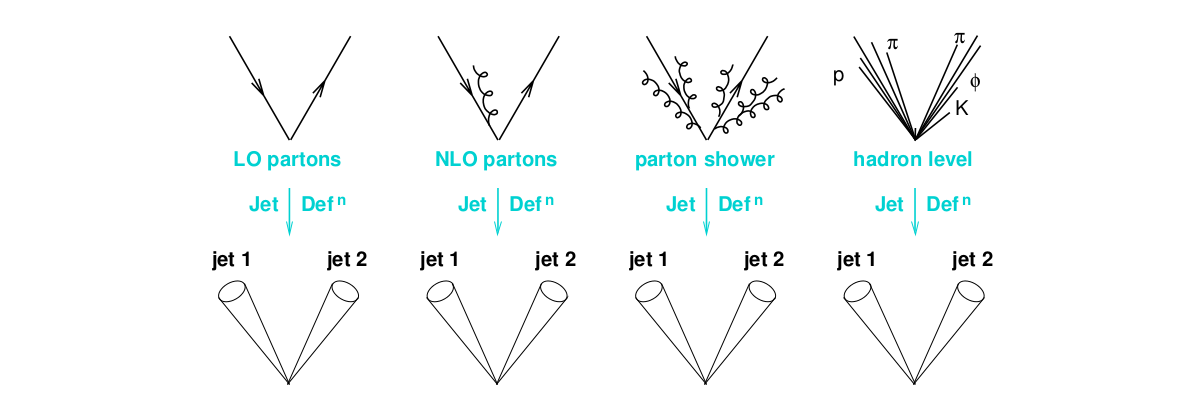
\includegraphics[width=1\textwidth]{Fig2/jetdefinition.png}
    \caption{The application of a jet definition to a variety of events that differ just through soft/collinear branching and hadronization should give identical jets in all cases~\cite{GavinLectures}.}
    \label{fig:jetdefinition}
  \end{center}
\end{figure}

Tradiontally, jet algorithms have been classified into two categories: cone algorithms and sequential recombination algorithms. 

Cone-like algorithms are based on the collinear nature of gluon radiation and the parton shower described above. The decay products of and emission from a hard quark or gluon will tend to form a cone of particles in the $\eta - \phi$ plane as they propagate.
% Then a cone of a suitable radius will capture these decay procuts.
An cone algorithm will work as follows~\footnote{This is how CMS cone algorithm, used for the preparation for the LHC running, works.}: first, it sorts all particles in the event according to their momentum, and identifies the one with largest $\pt$. This is referred to as seed particle. Then a cone of radius $R$ in  $\eta - \phi$ is drawn around the seed. The direction of the sum of the momenta of those particles is identified and if it doesn't coincide with the seed direction then the sum is used as a new seed direction, and iterates until the sum of the cone contents coincides withthe previus seed (this type of algorithm is cone ``iterative'' cone since it iterates the cone direction). This is how a stable cone is reached. A difficulty and major drawback in this procedure is the use of the transverse momentum of the particle to select the first seed. This definition is collinear unsafe, i.e. a splitting of the hardest particle into a nearly collinear pair can have the consequence that another, less hard particle, pointing in a different direction suddenly becomes the hardest in the event, leading to a different final set of jets. There are many other variants of cone algorithms, and nearly all suffer from problems of either collinear safety, or infrared safety (an extra soft particle creates a new seed, which can lead to an extra stable cone being found). A fix for these problems came in a algorithm called Seedless Infrared Safe Cone (SISCOne)~\cite{SISCone}.


Recombination algorithms, on the other hand, are both collinear and infrared safe. And for this reason, they can be used in calculations to any order in perturbation theory. The term recombination is used given that these algorithms work as if they were inverting the sequence of splittings of the parton shower. In general, recombination algorithms operate by successively combining pairs of particles using a distance metric, $d_{ij}$.  At hadron colliders, due to the fact that one of the incoming partons may continue along the beam, for every pair of particles this metric is compared to a so-called ``beam distance'', $d_{iB}$, and only when  $d_{ij}<d_{iB}$ the particle pair is combined and considered for subsequent clustering steps. 

ATLAS (and also CMS) has chosen anti-$k_t$~\cite{antiktalg} algorithm as the default jet algorithm for use in physics analysis.  This recombination algorithm as well as the Cambridge-Achen algorithm~\cite{CamAchen}, or C$/$A are extensions of the original $k_t$ algorithm developed for the analysis of multi-jet events at $e^+ e^-$ colliders~\cite{JADE} and subsequently extended for use at hadron colliders~\cite{kt2}~\cite{kt1}. In this thesis, the $k_t$ algorithm was used for jet substructure studies, see section~\ref{sec:substructure}.

The orginal $k_t$ algorithm implements the following (\ref{eqn:origkt}) distance metric between particles $i$ and $j$,

\begin{equation} 
d_{ij} = \frac{2E_i E_j (1-cos\theta_{ij}) }{Q^2}
\label{eqn:origkt}
\end{equation}

where $Q$ is the total energy in the event, $E_i$ is the energy of particle $i$ and $\theta_{ij}$ the angle between particles $i$ and $j$. In the collinear limit, $d_{ij}$ is related to the relative transverse momentum between particles $i$ and $j$ (hence the name $k_t$ algorithm), normalized to the total visible energy.
The particles are combined if the minimum $d_{ij}$, $d_min$, is below a certain threshold, $y_{cut}$.  The jet multiplicity depends on the value of $y_{cut}$, as a lower value will result in more soft or colliinear emissions surviving as jets. %This is thus the first definition of an ``event shape'', this threshold marks the transition between two-jet events and three-jet events.
As mentioned above, for hadron colliders, the notion of a beam distance is added. A distance scale, $\Delta R = \sqrt{\Delta y^2 +\Delta \phi^2}$, is introduced to define the typical radius for a jet, effectively replacing $y_{cut}$. In this case for every pair of particles a new distance is define, (\ref{eqn:kt}),

\begin{equation} 
d_{ij} = min(p^2_{ti},p^2_{tj}) \frac{\Delta R^2_{ij}}{R^2}
\label{eqn:kt}
\end{equation}

and the beam distance, $d_{iB}=p^2_{ti}$. %, in the way that when no particle j is found such that $\Delta R_{ij} < R$ then i is promoted to the status of a jet. 
The algorithm proceeds by searaching for the smallest of the $d_{ij}$ and the $d_{iB}$. If it is a $d_{ij}$ then particles $i$ and $j$ are recombined into a single new particles. If it is a $d_{iB}$ then $i$ is removed from the list of particles, and called a jet. This is repeated until no particles remain.

As opposed to cone algorithms, for the $k_t$ algorithm, the jets have quite irregular shapes, and particles with $\Delta R_{ij} > R$ can still be clustered within the jet. This is a problem when, for example, an irregularly shaped jet happens to extend into poorly instrumented detector regions. Another drawback of this definition is that soft particles are clustered first. This  has the potential to introduce complications when the detector noise of energy density fluctuations are large.

A feature of the $k_t$ algorithm that is attractive is that it not produces jets but also assigns a clustering sequence to the particles within the jet. It is possible then to undo the clustering and look inside the structure of the jet. This has been exploited in a range of QCD studies, and also in searches of hadronic decays of boosted massive particles  and will be used here for the search of two-pronged jets in gluon splitting.

The prescription above may be generalized beyond the $k_t$ algorithm. By inverting the power law in the particle distance metric, $d_{ij}$, the anti-$k_t$ algorithm is obtained. The particle distance metric used by this algorithm is,

\begin{equation} 
d_{ij} = min(p^{-2}_{ti},p^{-2}_{tj}) \frac{\Delta R^2_{ij}}{R^2}
\label{eqn:antikt}
\end{equation}

and the  beam distance, $d_{iB}=p^{-2}_{ti}$. This definition results in the clustering of the hardest emissions first. This has several benefits in the context of high-luminosity hadron collisions.

Note that the anti-$k_t$ algorithm does not provide useful information on jet substructureL if a jet contains two hard cores, then the $k_t$ (or C/A) algorithms first reconstruct those hard cores and merge the resulting two subjets. The anti-$k_t$ will often first cluster the harder of the two cores and then gradually aglomerate the contents of the second hard core.

These algorithms, and more, are implemented in {\sc Fastjet}~\cite{fastjet} software package for jet-finding. 


%------------------------------------------------------------------------
\subsection{Jet substructure and shape variables}\label{sec:substructure}
%------------------------------------------------------------------------

Jet substructure techniques attempt to extract additional information about a jet from a detailed study of its constituents (see chapter\ref{sec:reconstruction}). Although these methods have been first thought for distinguishing boosted hadronic objects like SM top quarks and $W/Z/$Higgs bosons from the background of jets initiated by light quarks and gluon, they have been used succesfully in other applications, including separating quark jets from gluon jets~\cite{PhysRevLett.107.172001} and identifying boosted decay producs in new physics~\cite{PhysRevD.82.095012}.






\subsubsection{$N$-subjettiness}

$N$-subjettiness is jet shape that describes the energy flow of a jet with respect to candidate subjet axes.  


exclusive $k_t$ algorithm~\cite{exclusivekt}.

$N$-jettiness~\cite{njetti}.

$N$-subjettiness~\cite{nsubjettiness}.

Minimizing $N$-subjettiness~\cite{mininsubjettiness}
